\documentclass[11pt,a4paper]{article}
\usepackage[margin=2cm]{geometry}
\usepackage{amsmath,amssymb,graphicx,booktabs,fancyhdr,hyperref}
\hypersetup{colorlinks=true,urlcolor=blue,linkcolor=black}
\pagestyle{fancy}\fancyhf{}\fancyhead[L]{EE 315 Assignment 10}\fancyhead[R]{Sreehari J. --- 240002073}\fancyfoot[C]{\thepage}
\setlength{\headheight}{14pt}\setlength{\parskip}{5pt}\setlength{\parindent}{0pt}
\newcommand{\captext}[1]{\begin{center}\small #1\end{center}}
\begin{document}
\begin{center}\large\textbf{EE 315 Assignment 10}\\[5pt]\Large\textbf{Transient Stability Assessment of a Nine-Bus System and Critical Clearing-Time Analysis}\end{center}
\begin{tabular}{ll}
\textbf{Course}&EE 315 -- Power Systems\\
\textbf{Assignment}&Project / Assignment 10\\
\textbf{Name}&Sreehari J. (Member 2)\\
\textbf{Project Lead}&Akarsh J\\
\textbf{Roll Number}&240002073\\
\textbf{Group}&04\\
\textbf{Implementation}&MATLAB simulation\\
\textbf{Project Files}&\href{https://github.com/pacificblaster1708/PowerSystems-Project-10}{GitHub: PowerSystems-Project-10}\\
\textbf{Website}&\href{https://pacificblaster1708.github.io/PowerSystems-Project-10/}{View project website}
\end{tabular}
\vspace{10pt}\hrule
\section{Group Members}
\begin{center}\begin{tabular}{lll}\toprule Member&Roll Number&Name\\\midrule
Member 1&240002007&Akarsh J (Project Lead)\\
Member 2&240002073&Sreehari J.\\
Member 3&240002043&Naman V Shetty\\
Member 4&240002037&Mayur Soni\\
Member 5&240002017&Bhasuru Nikhil\\
Member 6&240002069&Ridhi Shakkar\\\bottomrule\end{tabular}\end{center}
\section{Introduction}
Transient stability concerns the ability of synchronous generators to remain in synchronism after a large disturbance. A fault changes the electrical power transferred through the network. The resulting imbalance between mechanical input and electrical output accelerates or decelerates the generator rotors. Clearing the fault changes the network again, and the subsequent rotor motion determines whether relative angles remain bounded.

This project studies a single-line-to-ground (SLG) fault in a three-generator, nine-bus system. The fault resistance is the last digit of roll number 240002073:
\[R_f=3\ \Omega.\]
The initial operating point is calculated, the unbalanced fault is represented using sequence networks, and the swing equations are integrated for different fault durations. The objective is to search for a critical clearing time (CCT), defined for the chosen event and operating point as the limiting fault duration separating acceptable and unacceptable rotor-angle responses.

The study was implemented and simulated in MATLAB. All numerical results presented here were obtained from the MATLAB simulations.
\newpage
\section{System Modelling}
\subsection{Network Configuration}
The network is adapted from MATPOWER case9. It contains three generators, three load buses and nine branches. The topology, branch reactances, line charging and power schedules are retained; branch resistances are neglected in accordance with the classical stability assumptions. The assigned fault resistance remains present.
\begin{center}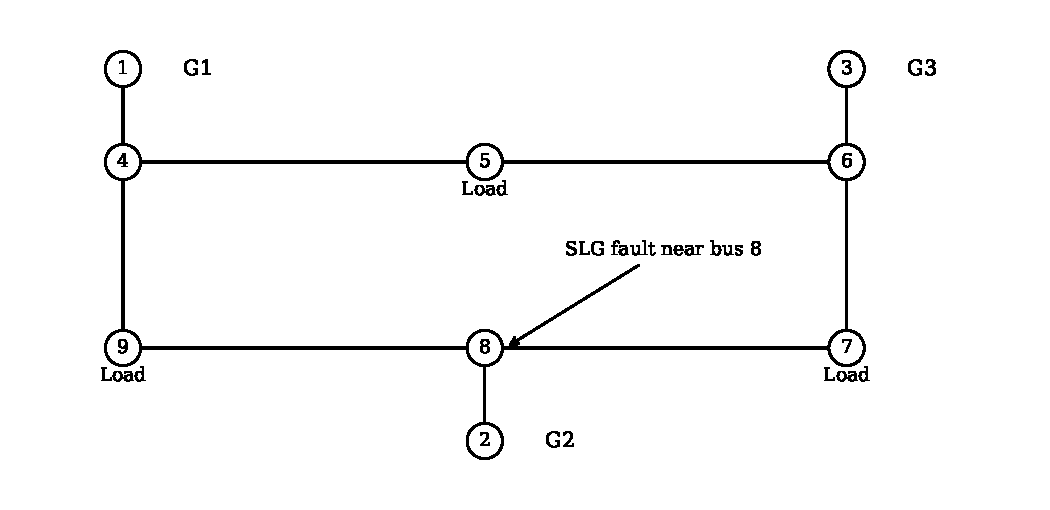
\includegraphics[width=.9\linewidth]{assets/network.pdf}\end{center}
\captext{Figure 1: Nine-bus network and the selected fault location. Bus numbers are shown in circles.}
\subsection{System and Generator Parameters}
\begin{center}\begin{tabular}{ll}\toprule Parameter&Value\\\midrule
System base&100 MVA\\ Transmission voltage base&345 kV, line-to-line\\ Frequency&50 Hz\\ Generator terminal voltage&1.0 pu\\ Loads at buses 5, 7 and 9&$90+j30$, $100+j35$, $125+j50$ MVA\\ Scheduled generation G2 / G3&163 MW / 85 MW\\ Loading factor&1.0\\\bottomrule\end{tabular}\end{center}
\begin{center}\begin{tabular}{lrrr}\toprule Parameter&G1&G2&G3\\\midrule
$H$ on 100-MVA base (s)&23.64&6.40&3.01\\
$X_d'$ (pu)&0.0608&0.1198&0.1813\\
Damping coefficient&0&0&0\\
Initial $P_m$ (pu)&0.670&1.630&0.850\\\bottomrule\end{tabular}\end{center}
The inertia and transient-reactance values are adopted study inputs. Mechanical input and internal-voltage magnitudes are held constant. Loads are represented by constant admittances during the disturbance. Governor, excitation-control and electromagnetic-transient dynamics are not included.
\newpage
\subsection{Branch and Sequence Data}
\begin{center}\begin{tabular}{lrrr}\toprule Branch&$R_1$ (pu)&$X_1$ (pu)&Total $B_1$ (pu)\\\midrule
1--4&0&.0576&0\\4--5&0&.0920&.158\\5--6&0&.1700&.358\\3--6&0&.0586&0\\6--7&0&.1008&.209\\7--8&0&.0720&.149\\8--2&0&.0625&0\\8--9&0&.1610&.306\\9--4&0&.0850&.176\\\bottomrule\end{tabular}\end{center}
The adopted line sequence relationships are $Z_2=Z_1$, $Z_0=3Z_1$ and $B_0=B_1/3$. Generator negative-sequence reactance is taken as $X_2=X_d'$. Step-up transformers have a generator-side delta winding and a grounded-wye transmission winding. Equivalent loads have equal positive- and negative-sequence impedances, with their zero-sequence paths open. These supplemental data specify the grounding and return paths needed for an SLG calculation.
\subsection{Fault Application and Clearing}
A phase-A-to-ground fault is applied on line 7--8, at 1\% of its length from bus 8, at $t_f=0.100$ s. An auxiliary algebraic node represents this point; it is not an additional physical bus in the original network. For a fault duration $\tau$, the clearing instant is $t_c=0.100+\tau$. Clearing opens line 7--8 at both ends, without automatic reclosure.
\section{Theoretical Analysis}
\subsection{Per-Unit Conversion}
Using the three-phase MVA base and line-to-line voltage base,
\[Z_{\rm base}=\frac{V_{\rm base}^2}{S_{\rm base}}=\frac{345^2}{100}=1190.25\ \Omega,
\qquad R_{f,\rm pu}=\frac{3}{1190.25}=0.00252048.\]
\subsection{Initial Operating Point and Load Representation}
A load-flow solution determines the bus voltages and generator currents. Bus 1 is the slack bus, buses 2 and 3 are voltage-controlled generation buses, and the remaining buses have specified net injections. The internal generator voltage and load admittance are
\[E_i'=V_i+jX_{di}'I_i,\qquad Y_{L,k}=\frac{P_{L,k}-jQ_{L,k}}{|V_k|^2}.\]
The mechanical power is initialized from pre-fault electrical power, so that each rotor starts at equilibrium. Since transmission resistances are zero, the scheduled active loads total 315 MW and the initial generation is $67+163+85=315$ MW.
\newpage
\subsection{SLG Fault and Network Reduction}
For a phase-A-to-ground fault, the boundary conditions are $I_b=I_c=0$ and $V_a=R_fI_a$. Symmetrical components give
\[I_0=I_1=I_2,\qquad I_a=3I_1.\]
The sequence networks are connected in series. In a Thevenin representation,
\[I_1=\frac{V_{\rm th}}{Z_{1,ff}+Z_{2,ff}+Z_{0,ff}+3R_{f,\rm pu}}.\]
For the time-domain classical model, the positive-sequence network is retained explicitly. Eliminating the passive negative- and zero-sequence networks gives a shunt at the fault point:
\[Y_{f,\rm eq}=\frac{1}{Z_{2,ff}+Z_{0,ff}+3R_{f,\rm pu}}.\]
The positive-sequence driving-point impedance is already represented by that network and is not added again in this shunt. Eliminating algebraic bus voltages produces the internal-generator admittance matrix
\[Y_{\rm red}=Y_{gg}-Y_{gb}Y_{bb}^{-1}Y_{bg}.\]
Separate reduced matrices are used before the fault, during the fault and after the line is opened. Generator electrical power is evaluated as
\[P_{e,i}=\operatorname{Re}\left\{E_i'\left(\sum_jY_{{\rm red},ij}E_j'\right)^*\right\}.\]
\subsection{Swing Equations}
For rotor angles in electrical radians, Lecture 30 gives
\[\frac{H_i}{\pi f}\frac{d^2\delta_i}{dt^2}=P_{m,i}-P_{e,i},\qquad
H_{i,\rm sys}=H_{i,\rm mach}\frac{S_{i,\rm mach}}{S_{\rm base}}.\]
Introducing the per-unit speed deviation $\Delta\omega_i$ yields
\[\dot\delta_i=2\pi f\Delta\omega_i,\qquad
\dot{\Delta\omega}_i=\frac{P_{m,i}-P_{e,i}}{2H_i}.\]
No damping term is included. The three angle states and three speed states are solved together, with electrical power recalculated at each integration stage.
\subsection{Clearing-Time Assessment}
The slide expression $t_{cr}=\sqrt{2H(\delta_{cr}-\delta_0)/(\pi fP_m)}$ applies when $P_e=0$ during the fault. That condition is not assumed for this SLG event; the coupled swing equations are integrated instead. Loss of synchronism is detected numerically when the unwrapped pairwise angle spread reaches $360^\circ$. Passing a finite observation window is a numerical test, not a proof of stability for all future time.
\newpage
\section{Simulation and Computational Procedure}
\subsection{Integration and Duration Search}
For the state equation $\dot x=F(x)$, fourth-order Runge--Kutta uses
\begin{align*}
k_1&=F(x_n),&k_2&=F(x_n+hk_1/2),\\
k_3&=F(x_n+hk_2/2),&k_4&=F(x_n+hk_3),\\
x_{n+1}&=x_n+\frac h6(k_1+2k_2+2k_3+k_4).
\end{align*}
The time step is shortened when necessary to land exactly on fault application or clearing. This prevents one integration step from mixing two network configurations.
\begin{enumerate}
\item Solve the pre-fault load flow and calculate internal generator voltages and load admittances.
\item Form pre-fault, fault-on and post-fault reduced networks.
\item Initialize the rotor angles from internal voltages and set speed deviations to zero.
\item Simulate a selected fault duration and observe the response for 20 s after clearing.
\item Record the largest pairwise angle spread and whether the $360^\circ$ threshold is reached.
\item Repeat for 61 durations from 0 to 3 s in 0.05 s increments.
\item If a passing/failing interval is found, refine it by bisection until its width is at most 0.001 s. If none is found, report that no finite CCT was identified in the sampled range.
\end{enumerate}
\subsection{MATLAB Implementation}
The standalone function is \texttt{Assignment10\_Sreehari\_G4\_M2.m}. To generate MATLAB outputs, run:
\begin{verbatim}
results = Assignment10_Sreehari_G4_M2;
\end{verbatim}
The function requires no additional toolbox. It saves a duration-scan CSV, two trajectory CSVs, a summary, a MAT file and a rotor-angle/speed figure in \texttt{results\_matlab/}. The settings are a 0.002 s integration step, 20 s post-clear observation and 0.001 s boundary tolerance. The default loading factor is 1.0 and $R_f=3\ \Omega$.
\subsection{Output Quantities}
Plots use the inertia-weighted centre-of-inertia angle:
\[\delta_{\rm COI}=\frac{\sum_iH_i\delta_i}{\sum_iH_i},\qquad
\delta_{i,\rm rel}=\delta_i-\delta_{\rm COI}.\]
The frequency deviation is $\Delta f_i=f\Delta\omega_i$. The detection quantity is $\max_i\delta_i-\min_i\delta_i$, calculated from unwrapped angles. Removing the common angle motion improves readability without changing the pairwise differences.
\newpage
\section{Simulation Results}
\subsection{Initial Bus Voltages}
\begin{center}\begin{tabular}{rrr}\toprule Bus&Voltage magnitude (pu)&Angle (degrees)\\\midrule
1 & 1.000000 & 0.0000 \\
2 & 1.000000 & 10.0228 \\
3 & 1.000000 & 5.1352 \\
4 & 0.993430 & -2.2263 \\
5 & 0.991343 & -3.7544 \\
6 & 1.001664 & 2.2848 \\
7 & 0.987696 & 0.9102 \\
8 & 0.992276 & 4.1300 \\
9 & 0.973556 & -4.1631 \\
\bottomrule\end{tabular}\end{center}
\captext{Table 1: Calculated pre-fault operating point, referenced to bus 1.}
The smallest initial voltage is 0.973556 pu at bus 9. The load-flow mismatch is $9.51\times10^{-11}$ pu. The initial accelerating power is zero to numerical precision because $P_m$ is initialized from the same pre-fault network.
\subsection{Response for a 0.100 s Fault}
\begin{center}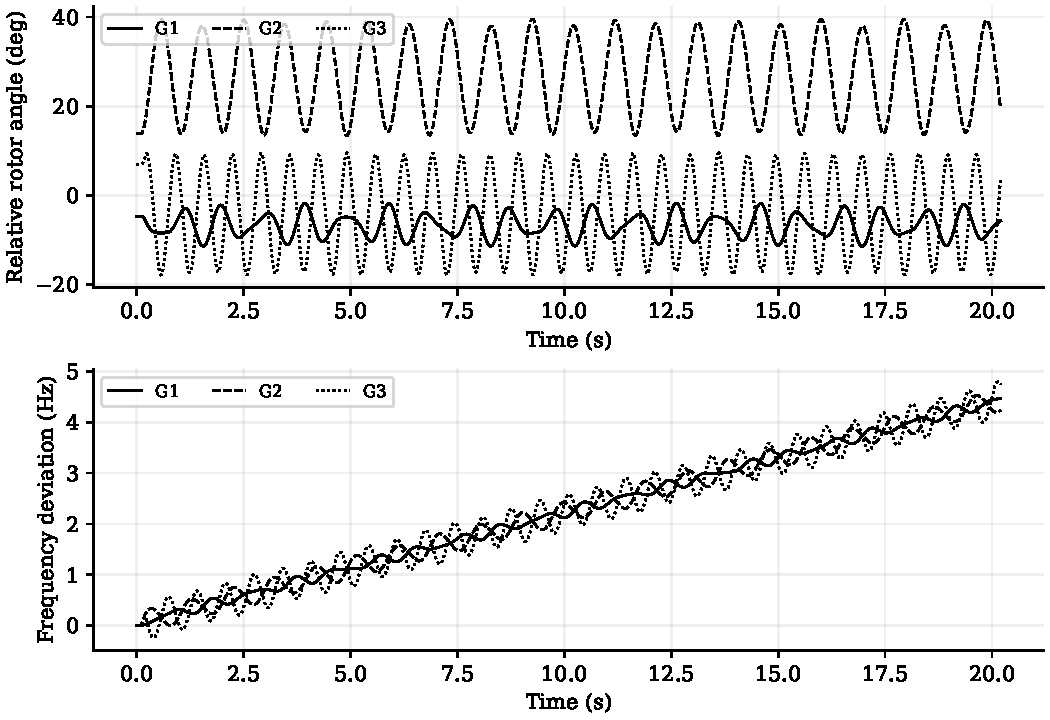
\includegraphics[width=.96\linewidth]{assets/short.pdf}\end{center}
\captext{Figure 2: Relative rotor angles and frequency deviations for clearing at $t=0.200$ s.}
The largest pairwise rotor-angle separation is $57.416^\circ$. The generators oscillate relative to one another without crossing the chosen loss-of-synchronism threshold during the observation window. The oscillations persist because damping is omitted.
\newpage
\subsection{Response for a 3.000 s Fault}
\begin{center}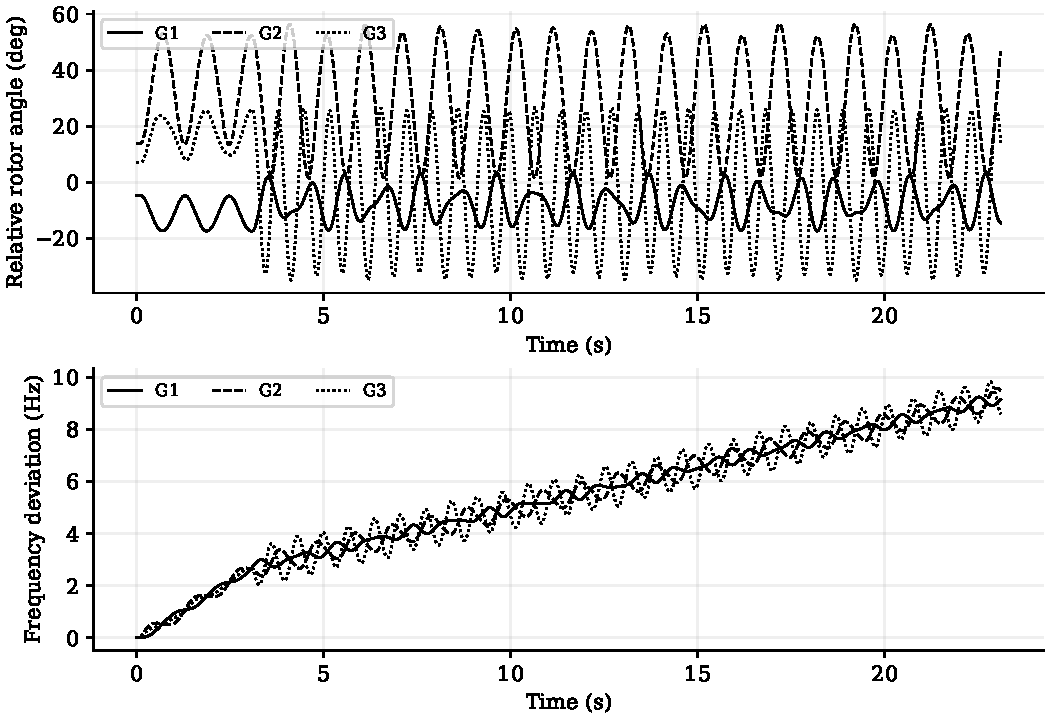
\includegraphics[width=.96\linewidth]{assets/long.pdf}\end{center}
\captext{Figure 3: Relative rotor angles and frequency deviations for clearing at $t=3.100$ s.}
For the 3 s fault, the peak pairwise separation is $91.294^\circ$. The relative rotor angles remain within the threshold, although common frequency drift is visible. Thus the angle test alone does not demonstrate acceptable frequency regulation.
\subsection{Duration-Scan Results}
\begin{center}\begin{tabular}{rrl}\toprule Fault duration (s)&Peak pairwise angle (degrees)&Angle test\\\midrule
0.00 & 54.264 & Pass \\
0.10 & 57.416 & Pass \\
0.50 & 88.832 & Pass \\
1.00 & 70.366 & Pass \\
1.50 & 75.166 & Pass \\
2.00 & 78.954 & Pass \\
2.50 & 70.366 & Pass \\
3.00 & 91.294 & Pass \\
\bottomrule\end{tabular}\end{center}
\captext{Table 2: Selected trials from the 61-case duration scan. Each trial includes 20 s after clearing.}
All 61 sampled durations pass. No passing/failing bracket is therefore available for bisection, and no finite CCT is identified within the sampled 0--3 s range.
\newpage
\subsection{Variation with Fault Duration}
\begin{center}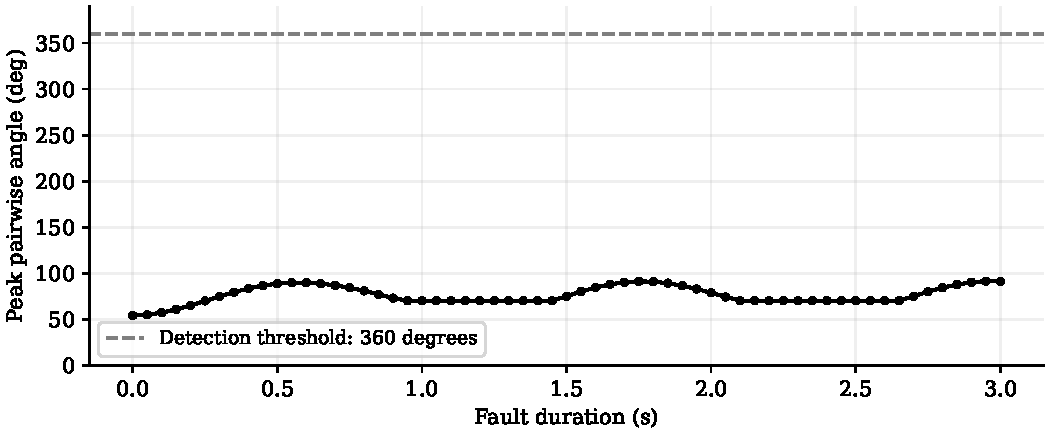
\includegraphics[width=.96\linewidth]{assets/scan.pdf}\end{center}
\captext{Figure 4: Peak pairwise rotor-angle separation over each complete trajectory.}
The response is not monotonic in fault duration: clearing occurs at different phases of the fault-on rotor oscillation, so the post-clear peak can rise or fall. The maximum observed value across the scan is 91.579 degrees at a fault duration of 2.95 s. All sampled peaks remain below the numerical threshold.
\subsection{Numerical Verification}
\begin{center}\begin{tabular}{p{.53\linewidth}p{.39\linewidth}}\toprule Check&Result\\\midrule
RK4 step reduced from 2 ms to 1 ms&No boundary in the full 0--3 s scan\\
Post-clear observation extended to 40 s&No boundary in the full 0--3 s scan\\
Independent Newton load flow&Maximum mismatch $6.11\times10^{-13}$ pu\\
Independent DOP853 integration&0, 0.1, 1 and 3 s trials pass\\
SLG condition $V_a=R_fI_a$&Residual $8.67\times10^{-18}$ pu\\\bottomrule\end{tabular}\end{center}
All reference calculations, integration and verification checks were carried out in MATLAB; the provided MATLAB function reproduces these results.
\section{Discussion and Conclusion}
For the specified normal-loading network, grounding arrangement and line 7--8 SLG event with $R_f=3\ \Omega$, all 61 tested durations pass the relative-angle criterion. The study therefore reports \textbf{no finite CCT identified within the sampled 0--3 s interval}. It does not infer infinite CCT or guarantee the outcome at every unsampled duration.

The classical model isolates rotor-angle behaviour. Fixed mechanical input and omitted governors permit common speed drift; this limits the physical accuracy of long-horizon trajectories evaluated with fixed-frequency network parameters. Voltage/reactive limits, excitation control, electromagnetic transients and negative-sequence heating or torque ripple are outside the model. The numerical result is consequently specific to these declared assumptions.

{\small\textbf{References.} EE 315 Lecture 27: SLG sequence networks; Lecture 30, pp. 3--7 and 17: swing equations, inertia conversion, classical assumptions and clearing time; Lecture 31: equal-area examples. Network data: \href{https://github.com/MATPOWER/matpower/blob/master/data/case9.m}{MATPOWER case9}.}
\end{document}
